\chapter{Results}
\label{ch:results}

\section{Reproduction and Verification of Results}
\label{ch:results-reproduction}

Given that this thesis draws heavily upon the research conducted by \cite{kotelnikov2022TabDDPMModellingTabular},
it was deemed absolutely necessary to first reproduce the original experiments and subsequently verify the authors findings,
prior to conducting any new experiments.
Fortunately, the publicly available code \cite{akim2023TabDDPMModellingTabular}, facilitated the replication of the experiments with relative ease.

The reproduction is limited to the adult dataset from \autoref{ch:methods-datasets} and to the machine learning efficacy computed with regards to a tuned CatBoost \cite{prokhorenkova2018CatBoostUnbiasedBoosting} model.

Firstly, a CatBoost model was tuned on the adult dataset, using the provided tuning script (tune\_evaluation\_model.py) [TODO: Drin lassen oder weg lassen?].
Next, for each sampling algorithm, a model was trained, according to the configuration files provided by the authors.
Each configuration file contains the parameters the authors found during hyperparameter tuning.
Hence, with the models respective pipeline.py script, the best found model from hyperparameter tuning could be trained and saved.
Finally, the trained CatBoost and trained sampling model were used in the evaluation script (eval\_seeds.py), which calculates and reports the results.

\begin{table}[h]
	\centering
	\begin{tabular}{l|c|c|r}
		\hline
		\textbf{Model}     & \textbf{Reproduction} & \textbf{Original} & \textbf{Difference} \\ \hline
		Real               & 0.815                 & 0.815             & 0                   \\ \hline
		TVAE$^{ml}$        & 0.780                 & 0.781             & -0.001              \\ \hline
		CTABGAN$^{ml}$     & 0.775                 & 0.783             & -0.008              \\ \hline
		CTABGAN+$^{ml}$    & 0.775                 & 0.772             & +0.003              \\ \hline
		SMOTE$^{ml}$       & 0.791                 & 0.791             & 0                   \\ \hline
		TabDDPM$^{ml}_{q}$ & 0.794                 & 0.795             & -0.001              \\ \hline
	\end{tabular}
	\caption[Reproduction of original Results]{Comparison of the CatBoost F1-score on synthetic datasets, created by different sampling models.
		F1-Scores of the reproduction experiments are compared against the results reported by the original authors \cite[Table 4, p. 8]{kotelnikov2022TabDDPMModellingTabular}.}
	\label{tab:reproduction}
\end{table}

\autoref{tab:reproduction} shows the computed F1-scores achieved by the CatBoost model when trained on different synthetic datasets generated by different sampling models.
The scores that could be reproduced are almost exactly the same as the scores reported by the original authors.
All differences are within the standard deviation reported by the authors, except for the CTABGAN-model.
It is unclear, why the CTABGAN-model score deviates in the reproduction experiment from the original score.
It is important to note, that minor modifications to the code or different python library versions have caused this alternation, which where required in order to train the model in the cloud environment, specified in \autoref{ch:methods-experimentalSetup}.

Therefore, the results as reported by the authors could be overall reproduced and verified.

\section{Metric Results}
\label{ch:results-Metric-results}

% QUALITATIVE vs QUANTITIVE

\subsection{Baseline Experiments}
\label{ch:Baseline}

After verification that the models are able to reproduce the machine-learning efficacy scores as reported,
their performance is additionally evaluated using the similarity evaluation as proposed in \autoref{ch:conceptualDesign-Evaluation}.
\autoref{tab:ml_baseline} shows the complete machine learning efficacy score results for the different sampling techniques:

\begin{table}[h]
	\centering
	\begin{tabular}{l|c|c|c}
		\hline
		\textbf{Model}     & \textbf{Accurarcy} & \textbf{F1}    & \textbf{ROC-AUC} \\ \hline
		Real               & 0.874              & 0.815          & 0.928            \\ \hline
		TVAE$^{ml}$        & 0.845              & 0.781          & 0.900            \\ \hline
		CTABGAN$^{ml}$     & 0.850              & 0.775          & 0.900            \\ \hline
		CTABGAN+$^{ml}$    & 0.855              & 0.775          & 0.907            \\ \hline
		SMOTE$^{ml}$       & 0.858              & 0.791          & 0.910            \\ \hline
		TabDDPM$^{ml}_{q}$ & \textbf{0.860}     & \textbf{0.794} & \textbf{0.913}   \\ \hline
	\end{tabular}
	\caption[Machine learning efficacy baseline]{Machine learning efficacy (CatBoost) baseline results.}
	\label{tab:ml_baseline}
\end{table}


In addition to the machine learning efficacy scores, the similarity scores of the TabSynDex metric are computed (\autoref{tab:sim_baseline}).

\begin{table}[h]
	\centering
	\begin{tabular}{lrrrrrr}
		\toprule
		\textbf{Model}     & \textbf{Similarity Score} & \textbf{Basic} & \textbf{Correlation} & \textbf{ML}    & \textbf{Support} & \textbf{pMSE}  \\
		\midrule
		Real               & 0.960                     & 0.992          & 0.943                & 0.998          & 0.984            & 0.882          \\
		TVAE$^{ml}$        & 0.658                     & 0.854          & 0.814                & 0.962          & 0.657            & 0.000          \\
		CTABGAN$^{ml}$     & 0.741                     & 0.940          & 0.832                & 0.984          & \textbf{0.947}   & 0.000          \\
		CTABGAN+$^{ml}$    & 0.750                     & 0.969          & 0.882                & 0.990          & 0.892            & 0.019          \\
		SMOTE$^{ml}$       & 0.723                     & 0.953          & 0.865                & \textbf{0.992} & 0.804            & 0.000          \\
		TabDDPM$^{ml}_{q}$ & \textbf{0.759}            & \textbf{0.973} & \textbf{0.919}       & \textbf{0.992} & 0.874            & \textbf{0.035} \\
		\bottomrule
	\end{tabular}
	\caption[Similarity baseline]{Similarity baseline results using the TabSynDex metrices. Similarity Score is the average of the other five scores. Best result is highlighted in bold}
	\label{tab:sim_baseline}
\end{table}

These baseline experiments show, that the Diffusion based synthesis approach outperforms other models not only in terms of machine learning efficacy, but also in terms of other metrics.
However, \autoref{tab:sim_baseline} shows that the CTABGAN models outperform TabDDPM in the Support coverage metric.
Additionally, it is worth mentioning that even though TabDDPM achieves the highest \gls{pmse} score, it is still extremely low and almost 0, which is the same for all other models.
The authors of \cite{chundawat2022UniversalMetricRobust} essentially confirm this observation.
During their experiments, the tested sampling techniques (various \gls{gan}-based approaches) also struggle to produce any synthetic data which achieves a \gls{pmse} score that is noticeably higher than 0.
\autoref{tab:sim_baseline} indicates, that this observation also holds for a diffusion based approach, which hyperparameters were tuned towards a machine learning efficacy score using a CatBoost model.

\subsection{Experiment 1: Adding Tabular Processing}
\label{ch:Experiment-1}

In the first set of experiments, the different tabular processing mechanism described in \autoref{ch:architecture-tabularProcessor-implementations} are evaluated.
For this, the tabular processing mechanisms have been added to the pipeline of TabDDPM, as described in the concept in \autoref{fig:Overall_changed}.
Consequently, the tuning (tune\_ddpm.py, see \autoref{ch:scripts}) of the diffusion model with the additional tabular processing was required.
The models hyperparameter have again been tuned towards the machine learning efficacy of a CatBoost model.

The results of the machine learning efficacy and TabSynDex metric results can be found in \autoref{tab:exp1-ml} and \autoref{tab:exp1-sim} respectively.
\begin{table}[h]
	\centering
	\begin{tabular}{lrrr}
		\toprule
		\textbf{Model}         & \textbf{Accurarcy} & \textbf{F1}    & \textbf{ROC-AUC} \\
		\midrule
		Real                   & 0.874              & 0.815          & 0.928            \\
		TabDDPM$^{ml}_{q}$     & 0.860              & 0.794          & 0.913            \\
		TabDDPM-BGM$^{ml}_{q}$ & \textbf{0.863}     & \textbf{0.798} & \textbf{0.916}   \\
		TabDDPM-FT$^{ml}_{q}$  & 0.785              & 0.552          & 0.821            \\
		\bottomrule
	\end{tabular}
	\caption[Experiment1-ML-Efficacy]{CatBoost Machine learning efficacy scores for different tabular processing techniques.}
	\label{tab:exp1-ml}
\end{table}

\begin{table}[h]
	\centering
	\begin{tabular}{lrrrrrr}
		\toprule
		\textbf{Model}         & \textbf{Similarity Score} & \textbf{Basic} & \textbf{Correlation} & \textbf{ML}    & \textbf{Support} & \textbf{pMSE}  \\
		\midrule
		Real                   & 0.960                     & 0.992          & 0.943                & 0.998          & 0.984            & 0.882          \\
		TabDDPM$^{ml}_{q}$     & \textbf{0.759}            & \textbf{0.973} & \textbf{0.919}       & 0.992          & 0.874            & \textbf{0.035} \\
		TabDDPM-BGM$^{ml}_{q}$ & 0.742                     & 0.964          & 0.918                & \textbf{0.996} & 0.831            & 0.000          \\
		TabDDPM-FT$^{ml}_{q}$  & 0.595                     & 0.495          & 0.648                & 0.869          & \textbf{0.963}   & 0.000          \\
		\bottomrule
	\end{tabular}
	\caption[Experiment1-Similarity]{TabSynDex evaluation metric scores for different tabular processing techniques.}
	\label{tab:exp1-sim}
\end{table}

Both evaluations show, that the additional \gls{bgm} tabular processing seems to increase the ML-efficacy scores.
All metrics in \autoref{tab:exp1-ml} are highest for the TabDDPM-BGM model and the ML efficacy score of TabSynDex (which makes use of different models)
is highest for TabDDPM-BGM as well, although only by a slight margin.
\autoref{tab:exp1-sim} indicates, that this increase seems to come at the cost of reduced performance in the other metrices, which are highest for the Basic-, Correlation- and pMSE-Score for the plain TabDDPM version.
TabDDPM-FT compares significantly worse than its counterparts in the Correlation and Basic similarity score.
Interestingly, TabDDPM-FT performance significantly better in the Support score than the other versions and approximately 13 percentage-points worse in terms of ML efficacy computed by the TabSynDex metric.
More details can be seen in the \autoref{tab:exp1-ml}, that shows that especially the F1 score from TabDDPM-FT is much worse than the F1 score of the other models.
Lastly, neither the \gls{bgm} nor the \gls{ft} tabular processing enable the diffusion model to produce synthetic data that is able to increase the \gls{pmse} score.


\subsection{Experiment 2: Similarity Hyperparameter optimization}
\label{ch:Experiment-2}

The second set of experiments are very similar to the first experiments.
Instead of tuning the models hyperparameters after the machine learning efficacy, as proposed by the original authors,
the models hyperparameters are tuned after the TabSynDex similarity score.

The results of the machine learning efficacy and TabSynDex metric results can be found in \autoref{tab:exp2-ml} and \autoref{tab:exp2-sim} respectively.

TODO FT simTune; ctabgan+simTUne

\begin{table}[h]
	\centering
	\begin{tabular}{lrrr}
		\toprule
		\textbf{Model}        & \textbf{Accurarcy} & \textbf{F1}    & \textbf{ROC-AUC} \\
		\midrule
		Real                  & 0.874              & 0.815          & 0.928            \\
		TabDDPM$^{s}_{q}$     & 0.856              & 0.782          & 0.908            \\
		TabDDPM-BGM$^{s}_{q}$ & \textbf{0.859}     & \textbf{0.792} & \textbf{0.911}   \\
		TabDDPM-FT$^{s}_{q}$  & 0.767              & 0.450          & 0.712            \\
		CTABGAN$^{s}$         & 0.850              & 0.776          & 0.900            \\
		TVAE$^{s}$            & 0.845              & 0.780          & 0.900            \\
		\bottomrule
	\end{tabular}
	\caption[Experiment2-ML-Efficacy]{CatBoost Machine learning efficacy scores for different tabular processing techniques which hyperparameter have been tuned towards the TabSynDex similarity score.}
	\label{tab:exp2-ml}
\end{table}

\begin{table}[h]
	\centering
	\begin{tabular}{lrrrrrr}
		\toprule
		\textbf{Model}        & \textbf{Similarity Score} & \textbf{Basic} & \textbf{Correlation} & \textbf{ML}    & \textbf{Support} & \textbf{pMSE}  \\
		\midrule
		Real                  & 0.960                     & 0.992          & 0.943                & 0.998          & 0.984            & 0.882          \\
		TabDDPM$^{s}_{q}$     & 0.852                     & 0.976          & \textbf{0.921}       & \textbf{0.991} & 0.952            & 0.420          \\
		TabDDPM-BGM$^{s}_{q}$ & \textbf{0.857}            & \textbf{0.982} & 0.858                & \textbf{0.991} & 0.920            & \textbf{0.532} \\
		TabDDPM-FT$^{s}_{q}$  & 0.589                     & 0.513          & 0.620                & 0.819          & \textbf{0.992}   & 0.000          \\
		CTABGAN$^{s}$         & 0.740                     & 0.938          & 0.833                & 0.984          & 0.947            & 0.000          \\
		TVAE$^{s}$            & 0.658                     & 0.856          & 0.815                & 0.962          & 0.656            & 0.000          \\
		\bottomrule
	\end{tabular}
	\caption[Experiment2-Similarity]{TabSynDex evaluation metric scores for different tabular processing techniques which hyperparameter have been tuned towards the TabSynDex similarity score.}
	\label{tab:exp2-sim}
\end{table}

The results show, that TabDDPM-BGM outperforms all other models in terms of the CatBoost machine learning efficacy and is on pair with TabDDPM in the TabSynDex ML-efficacy score.
TabDDPM-BGM also has the highest overall Similarity Score and achieves the highest Basic score and \gls{pmse} score.
The simpler TabDDPM however outperforms its \gls{bgm} counterpart in terms of Correlation and Support score.
Overall, TabDDPM achieves comparable performance to TabDDPM-BGM on all metrics, with the biggest difference in the \gls{pmse} score of - 11 percentage points.
TabDDPM-FT performance significantly worse than all other TabDDPM variants in all metrics except the support score.
On the one hand, it seems to be the case that hyperparameter tuning after the similarity score does have a big influence on the TabDDPM and TabDDPM-BGM models \gls{pmse} score.
On the other hand, this hyperparameter tuning did not affect the \gls{pmse} score of the other tested model, the CTABGAN, TVAE or the TabDDPM-FT.

\subsection[]{Experiment 3: Exchanging the Normalization}
\label{ch:Experiment-3}

So far, all TabDDPM models received data, that was normalize according to the quantile-transform function (applied after tabular processing), as proposed in \cite{kotelnikov2022TabDDPMModellingTabular}.
In a third experiment, it will be investigated how the models perform, when their quantile-transform function is replaced by a more simple MinMax-scaler, as explained in \autoref{sec:dataNormalization}.
Based upon the performance of the model variants so far, only the plain TabDDPM and TabDDPM-BGM, tuned after the similarity score have been investigated, since the performance of TabDDPM-FT was noticeably worse.


\begin{table}[h]
	\centering
	\begin{tabular}{lrrr}
		\toprule
		\textbf{Model}        & \textbf{Accurarcy} & \textbf{F1}    & \textbf{ROC-AUC} \\
		\midrule
		Real                  & 0.874              & 0.815          & 0.928            \\
		TabDDPM$^{s}_{m}$     & 0.856              & 0.778          & \textbf{0.910}   \\
		TabDDPM-BGM$^{s}_{m}$ & \textbf{0.857}     & \textbf{0.787} & 0.909            \\
		\bottomrule
	\end{tabular}
	\caption[Experiment3-ML-Efficacy]{CatBoost Machine learning efficacy scores for different tabular processing techniques which hyperparameter have been tuned towards the TabSynDex similarity score
		and the data was transformed according to a MinMax-scaler.}
	\label{tab:exp3-ml}
\end{table}

\begin{table}[h]
	\centering
	\begin{tabular}{lrrrrrr}
		\toprule
		\textbf{Model}        & \textbf{Similarity Score} & \textbf{Basic} & \textbf{Correlation} & \textbf{ML}    & \textbf{Support} & \textbf{pMSE}  \\
		\midrule
		Real                  & 0.960                     & 0.992          & 0.943                & 0.998          & 0.984            & 0.882          \\
		TabDDPM$^{s}_{m}$     & \textbf{0.869}            & 0.938          & \textbf{0.930}       & 0.990          & \textbf{0.928}   & \textbf{0.558} \\
		TabDDPM-BGM$^{s}_{m}$ & 0.856                     & \textbf{0.981} & 0.913                & \textbf{0.992} & 0.915            & 0.476          \\
		\bottomrule
	\end{tabular}
	\caption[Experiment3-Similarity]{TabSynDex evaluation metric scores for different tabular processing techniques which hyperparameter have been tuned towards the TabSynDex similarity score
		and the data was transformed according to a MinMax-scaler.}
	\label{tab:exp3-sim}
\end{table}

Given the results in \autoref{tab:exp3-ml} and \autoref{tab:exp3-sim} it seems to be the case that TabDDPM-BGM outperforms TabDDPM in terms of ML-efficacy and the Basic score, but only by a slight margin.
TabDDPM, on the other hand, achieves a higher overall similarity score, mainly due to the superior performance in the Correlation, Support and pMSE-score.


\section{Visual Results}
\label{ch:results-Visual}

Several plots have been produced accroding to the methodology of \cite{brenninkmeijer2019GenerationEvaluationTabular}.
This section will cover which plots have been produced and how the plots for different model versions are different.

\subsection[]{Correlation Difference Matrix}

To get an intuition on how well correlations within the dataset are reproduced, correlation matrices have been computed.
The correlation matrix for the synthetic dataset has been subtracted from the correlation matrix of the real dataset in order to produce a correlation difference matrix.
The smaller the difference, the more similar are the correlations within the synthetic dataset to the correlations within the real dataset.

Looking at the correlations matrix differences in \autoref{fig:corr_base} for the baseline models that are not diffusion based, one can see that the CTABGAN+$^{ml}$ and SMOTE approaches have the smallest
correlation matrix difference.
However, the diffusion model TabDDPM$^{ml}$ produces the matrix with the smallest overall differences.

\begin{figure}[h]
	\centering
	\begin{subfigure}{0.3\textwidth}
		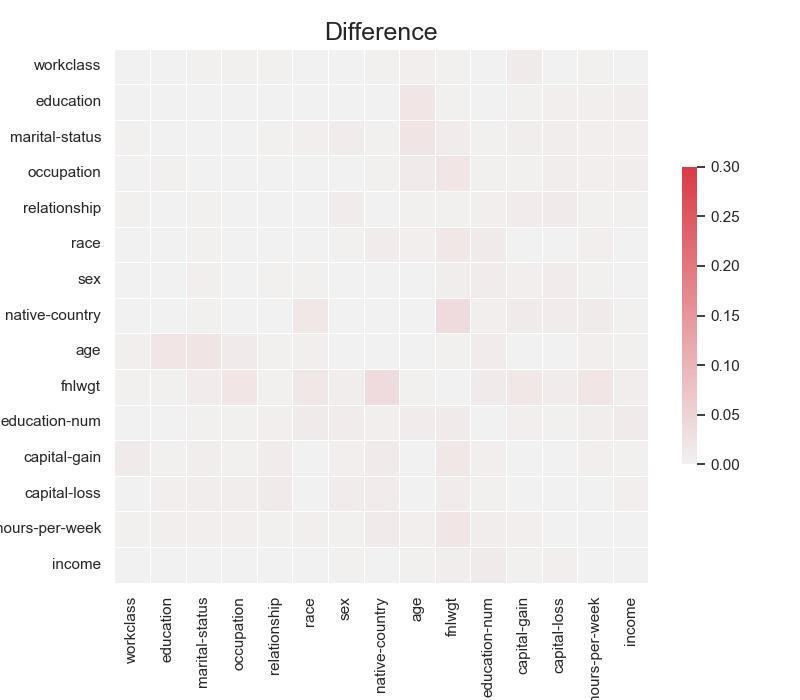
\includegraphics[width=\textwidth]{images/correlation_difference/real.jpg}
		\caption{Real}

	\end{subfigure}
	\hfill
	\begin{subfigure}{0.3\textwidth}
		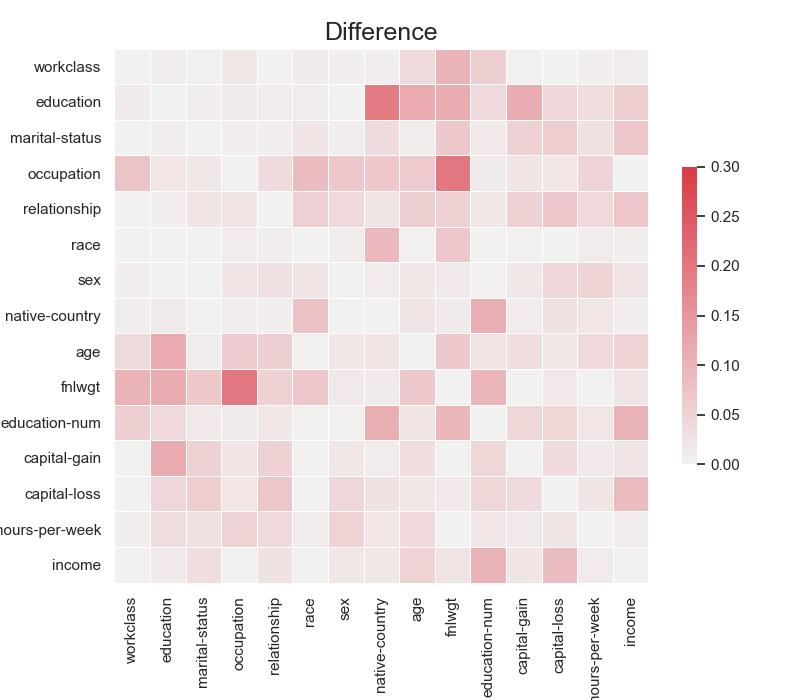
\includegraphics[width=\textwidth]{images/correlation_difference/tvae.jpg}
		\caption{TVAE$^{ml}$}

	\end{subfigure}
	\hfill
	\begin{subfigure}{0.3\textwidth}
		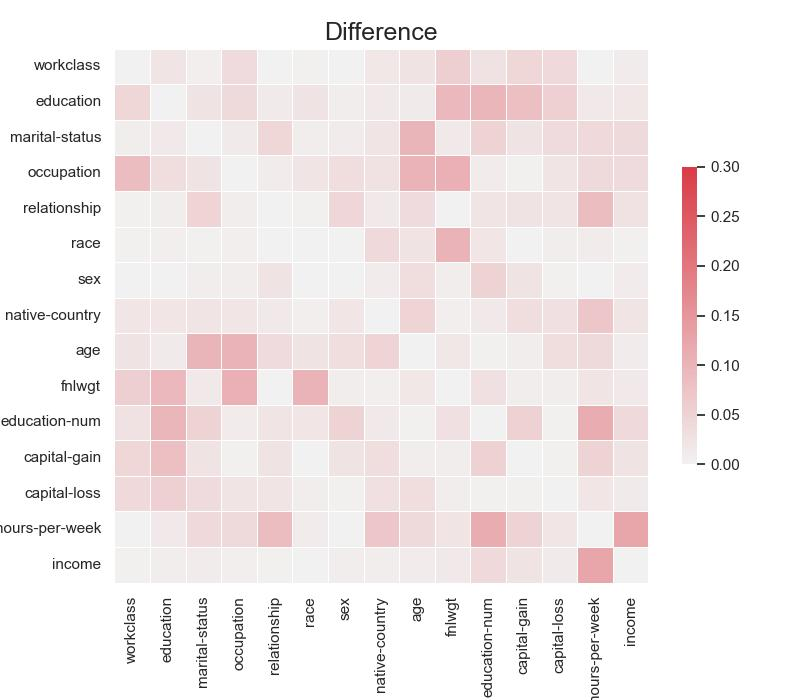
\includegraphics[width=\textwidth]{images/correlation_difference/ctabgan.jpg}
		\caption{CTABGAN$^{ml}$}
	\end{subfigure}

	\begin{subfigure}{0.3\textwidth}
		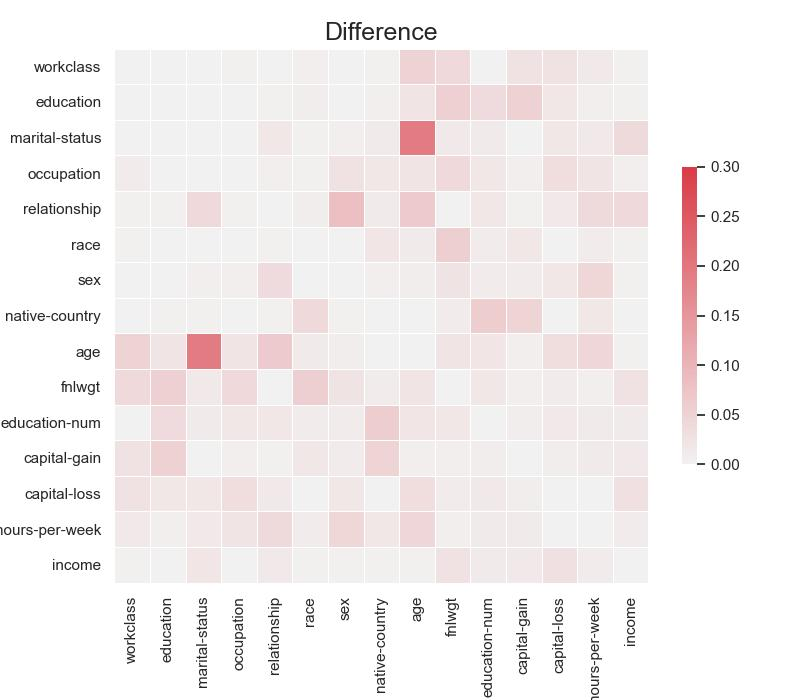
\includegraphics[width=\textwidth]{images/correlation_difference/ctabgan+.jpg}
		\caption{CTABGAN+$^{ml}$}

	\end{subfigure}
	\begin{subfigure}{0.3\textwidth}
		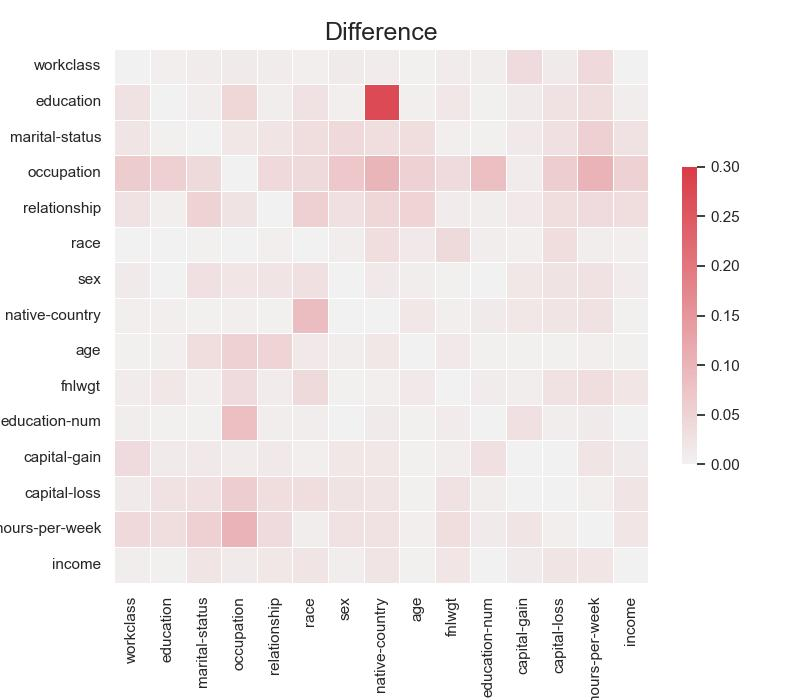
\includegraphics[width=\textwidth]{images/correlation_difference/smote.jpg}
		\caption{SMOTE}

	\end{subfigure}
	\begin{subfigure}{0.3\textwidth}
		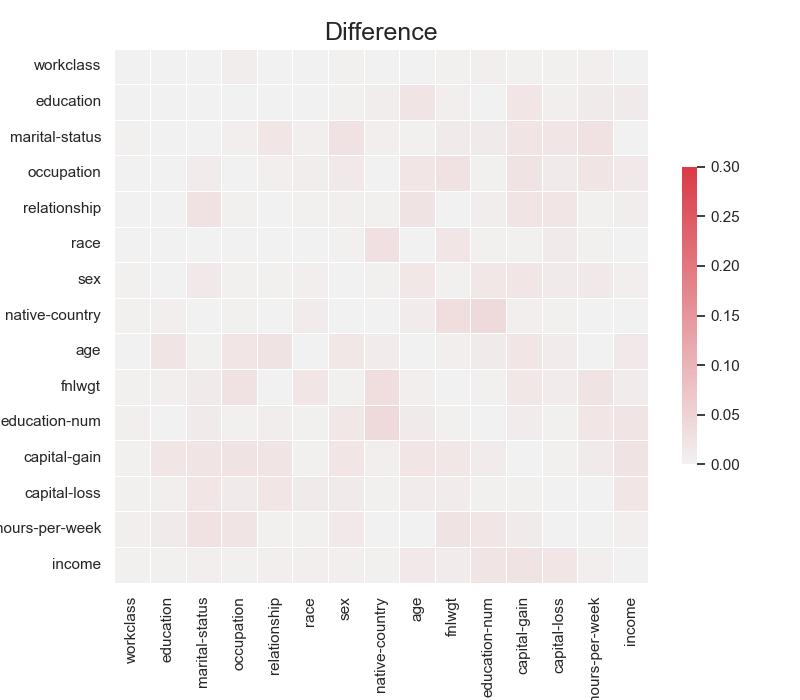
\includegraphics[width=\textwidth]{images/correlation_difference/tab-ddpm.jpg}
		\caption{TabDDPM$^{ml}_q$}

	\end{subfigure}
	\caption{Correlation Matrix difference for Baseline models.}
	\label{fig:corr_base}
\end{figure}


\begin{figure}[h]
	\begin{subfigure}{0.3\textwidth}
		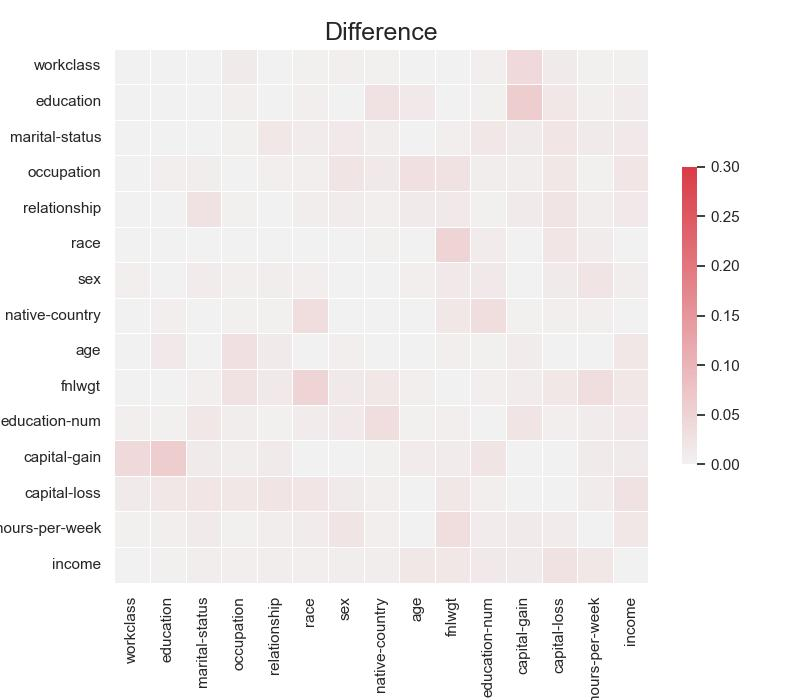
\includegraphics[width=\textwidth]{images/correlation_difference/tab-ddpm-bgm.jpg}
		\caption{TabDDPM-BGM$^{ml}_q$}
	\end{subfigure}
	\hfill
	\begin{subfigure}{0.3\textwidth}
		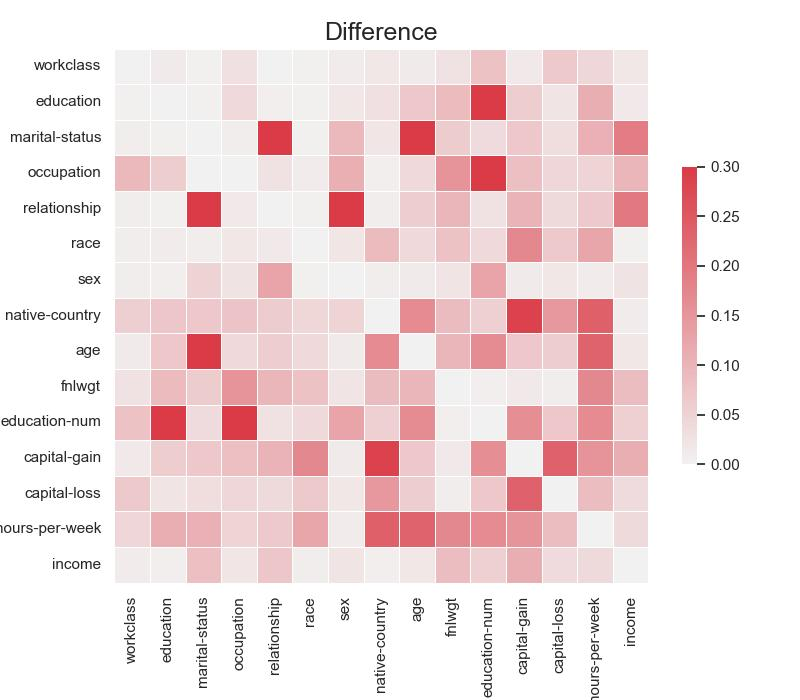
\includegraphics[width=\textwidth]{images/correlation_difference/tab-ddpm-ft.jpg}
		\caption{TabDDPM-FT$^{ml}_q$}
	\end{subfigure}
	\hfill
	\begin{subfigure}{0.3\textwidth}
		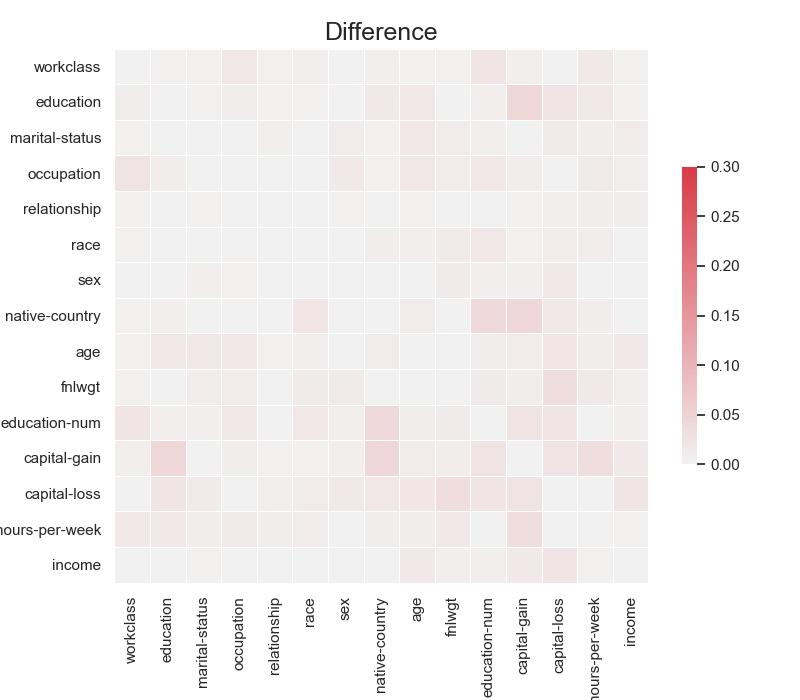
\includegraphics[width=\textwidth]{images/correlation_difference/tab-ddpm-bgm-simTune-minmax.jpg}
		\caption{TabDDPM-BGM$^{s}_m$}
	\end{subfigure}
	\caption{Correlation Matrix difference from selected experiment models.}
	\label{fig:corr_diffusion}
\end{figure}



\autoref{fig:corr_diffusion} shows that while the TabDDPM-BGM$^{ml}$ are able to produce small correlation differences, the TabDDPM-FT$^{ml}$ is not able to reproduce
the correlation matrix of the real dataset.
The overall best correlation difference matrix is produced by TabDDPM$^{s}_m$, which is also reflected in their TabSynDex correlation score in \autoref{tab:exp3-sim}, which is highest across all model versions.
Other model versions matrices do not show any noteworthy changes and are displayed in \autoref{fig_a:corr_diff}.

\subsection[]{Principle Component Analysis}
\label{ch:results-pca}

A \gls{pca} is a dimensionality reduction technique, that converts a dataset onto principal components \cite{brenninkmeijer2019GenerationEvaluationTabular}.
The components are then sorted according to the amount of variance from the original dataset each component is able to capture.
The following visualizations map the first two principal components, \ie the components that capture the most variance from data.


\begin{figure}[h]
	\centering
	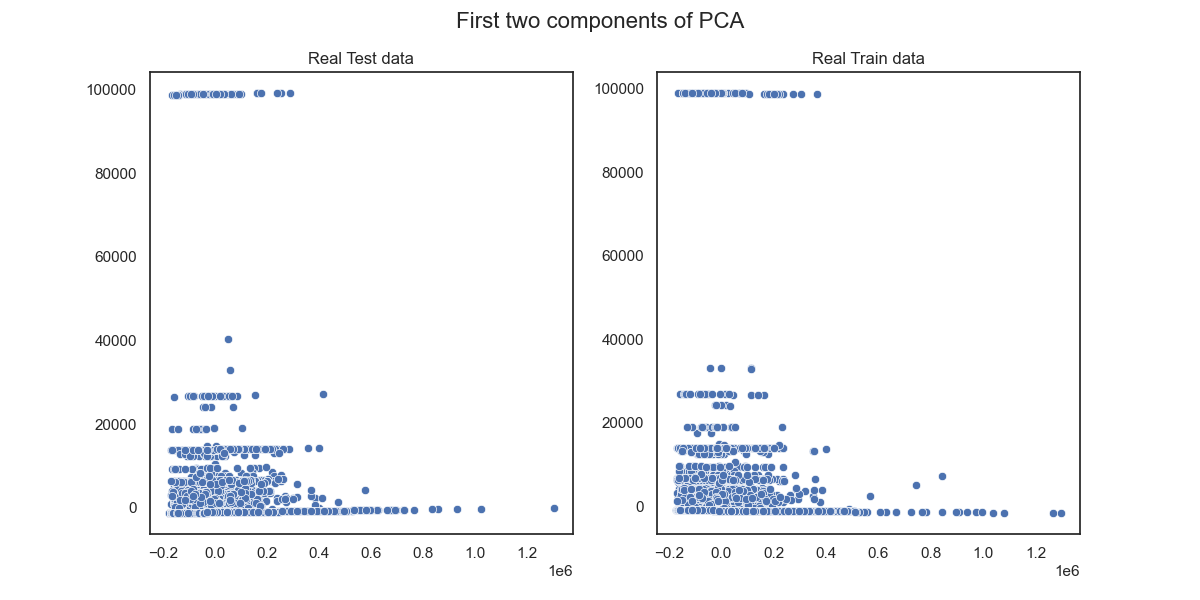
\includegraphics[width=0.6\textwidth]{images/pca/pca.png}
	\caption{\gls{pca} for the real training and testing dataset}
	\label{fig:pca}
\end{figure}

\autoref{fig:pca} shows the two \gls{pca} plots that display the fist two principle components from the real training and testing dataset.
One can see that the majority of values in the plots are scatter around the lower left corner (for $y<=40000$) with two accumulations of values spreading along the $x$-axis around $y=100000$ and $y=0$.
The goal of the synthetic data generation method is to produce synthetic data whose \gls{pca} plot is similar to the \gls{pca} plot of the real testing dataset.

\begin{figure}[h]
	\centering
	\begin{subfigure}{0.3\textwidth}
		\centering
		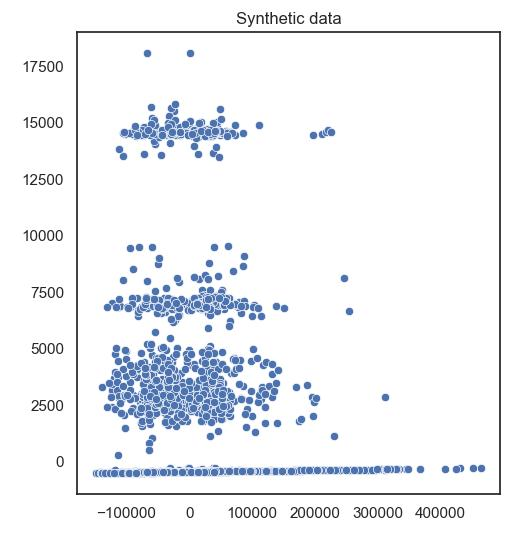
\includegraphics[width=\textwidth]{images/pca/tvae.jpg}
		\caption{TVAE$^{ml}$}
	\end{subfigure}
	\begin{subfigure}{0.3\textwidth}
		\centering
		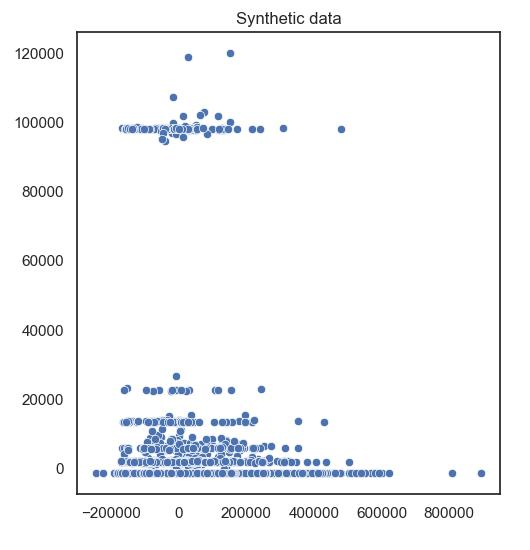
\includegraphics[width=\textwidth]{images/pca/ctabgan.jpg}
		\caption{CTABGAN$^{ml}$}
	\end{subfigure}
	\begin{subfigure}{0.3\textwidth}
		\centering
		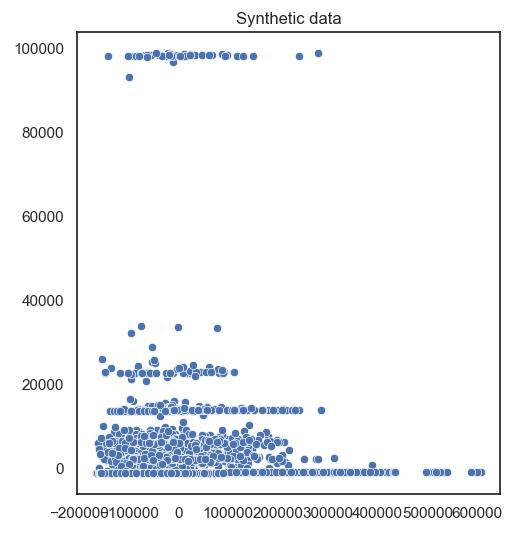
\includegraphics[width=\textwidth]{images/pca/ctabgan+.jpg}
		\caption{CTABGAN+$^{ml}$}
	\end{subfigure}
	\begin{subfigure}{0.3\textwidth}
		\centering
		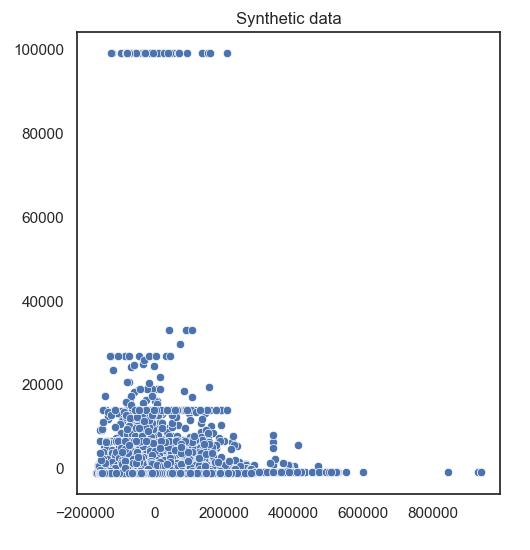
\includegraphics[width=\textwidth]{images/pca/smote.jpg}
		\caption{SMOTE}
	\end{subfigure}
	\begin{subfigure}{0.3\textwidth}
		\centering
		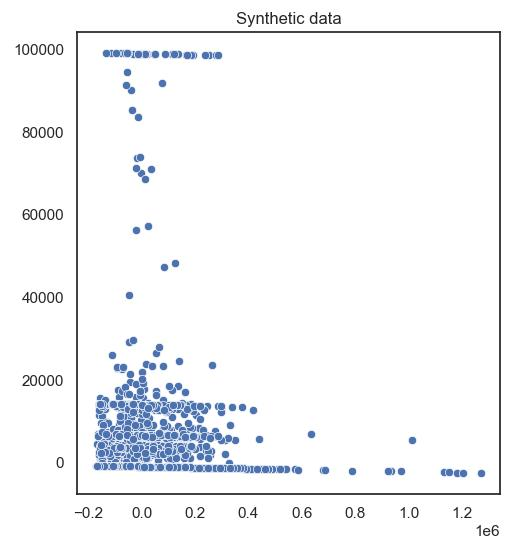
\includegraphics[width=\textwidth]{images/pca/tab-ddpm.jpg}
		\caption{TabDDPM$^{ml}_q$}
	\end{subfigure}
	\caption{\gls{pca} for Baseline models.}
	\label{fig:pca_base}
\end{figure}

\autoref{fig:pca_base} shows the \gls{pca} plots for the different baseline models. All plots show some similarity with the \gls{pca}-plot from the original dataset,
except for the TVAE model.

\begin{figure}[h]
	\centering
	\begin{subfigure}{0.2\textwidth}
		\centering
		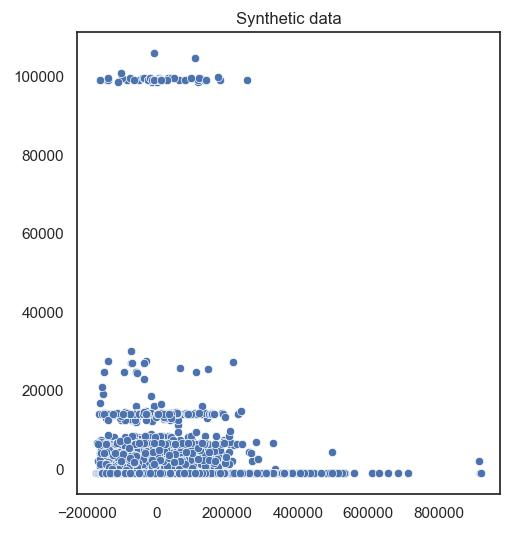
\includegraphics[width=\textwidth]{images/pca/tab-ddpm-bgm.jpg}
		\caption{TabDDPM-BGM$^{ml}_q$}
	\end{subfigure}
	\begin{subfigure}{0.2\textwidth}
		\centering
		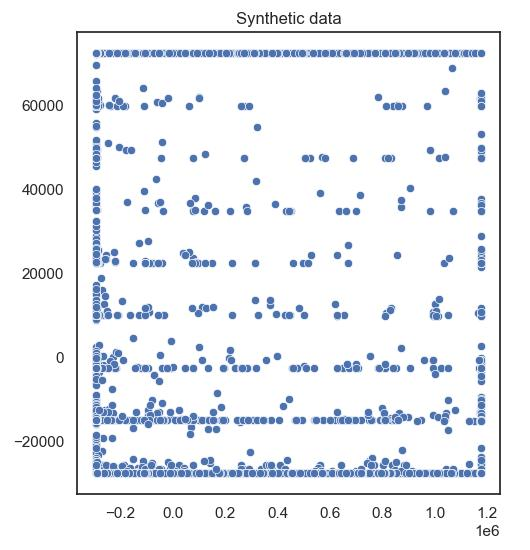
\includegraphics[width=\textwidth]{images/pca/tab-ddpm-ft.jpg}
		\caption{TabDDPM-FT$^{ml}_q$}
	\end{subfigure}
	\begin{subfigure}{0.2\textwidth}
		\centering
		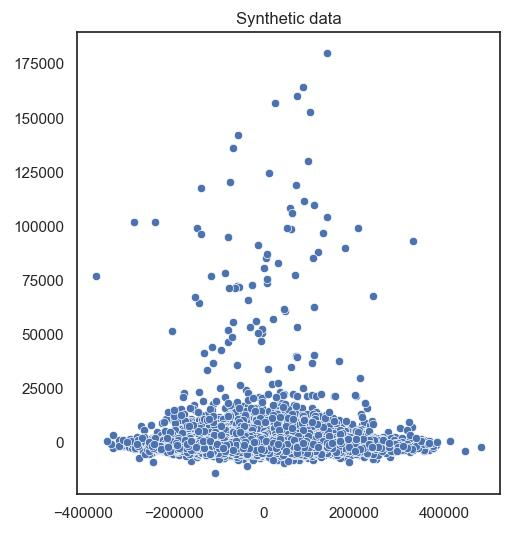
\includegraphics[width=\textwidth]{images/pca/tab-ddpm-simTune-minmax.jpg}
		\caption{TabDDPM$^{s}_m$}
	\end{subfigure}
	\begin{subfigure}{0.2\textwidth}
		\centering
		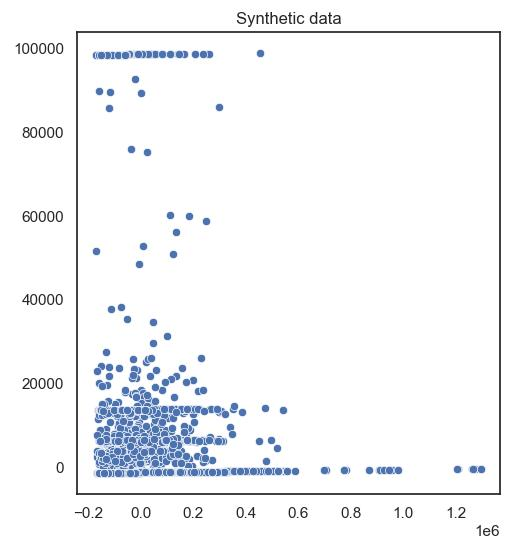
\includegraphics[width=\textwidth]{images/pca/tab-ddpm-simTune.jpg}
		\caption{TabDDPM$^{s}_q$}
	\end{subfigure}
	\caption{Correlation Matrix difference from selected experiment models.}
	\label{fig:pca_diffusion}
\end{figure}

Only the \gls{bgm} tabular processing mechanism seems to be able to produce a realistic \gls{pca}-plot.
Additionally, the Minmax scaling seems to have an effect on the \gls{pca}-plot for the TabDDPM model, however,
this did not affect the TabDDPM-BGM model that made use of Minmax scaling (\autoref{fig_a:pca_TabDDPMBM}).
This \gls{pca}-plot and the remaining model versions plots can be found at \autoref{A:pca}.

\subsection[]{Distribution Plot}
\label{ch:results-Distr}





\section{Analysis}
\label{ch:results-analysis}
%-------------------------------------------------------------------------


TODO: Continue here
\begin{table}[h]
	\centering
	\caption{Comparison of Model A and Model B}
	\label{tab:model-comparison}
	\begin{tabular}{|l|ccc|ccc|}
		\toprule
		\multirow{2}{*}{\textbf{Metrics}} & \multicolumn{3}{c|}{\textbf{TabDDPM}} & \multicolumn{3}{c|}{\textbf{TabDDPM-BGM}}                                                                                      \\ \cline{2-7}
		                                  & \textbf{ML-Efficacy}                  & \textbf{Similarity Score}                 & \textbf{Diff.} & \textbf{ML-Efficacy} & \textbf{Similarity Score} & \textbf{Diff.} \\
		\midrule
		\multicolumn{1}{|l|}{Accurarcy}   & 0.82                                  & 0.73                                      & +0.            & 0.76                 & 0.81                      & +0.            \\
		\multicolumn{1}{|l|}{Metric 2}    & 0.69                                  & 0.64                                      & +0.            & 0.72                 & 0.71                      & +0.            \\
		\multicolumn{1}{|l|}{Metric 3}    & 0.91                                  & 0.88                                      & +0.            & 0.89                 & 0.86                      & +0.            \\
		\bottomrule
	\end{tabular}
\end{table}



The tuning of the hyperparameters had a significant effect on the performance of the different models.

